
\documentclass[11pt]{article}
\usepackage[margin=1in]{geometry}
\usepackage{amsmath,amssymb}
\usepackage{graphicx}
\usepackage{booktabs}
\usepackage{array}
\usepackage{xcolor}
\usepackage{hyperref}
\hypersetup{colorlinks=true,linkcolor=blue,urlcolor=blue,citecolor=blue}
\setlength{\parskip}{0.6em}
\setlength{\parindent}{0pt}
\title{Spherical Cyclic Time v2.1-E\\Public Patch After Transfer Route Decision}
\author{Internal technical addendum}
\date{2026-07-04}
\begin{document}
\maketitle

\begin{abstract}
This addendum updates the public transfer-kernel language of \emph{Spherical Cyclic Time} after the v2.0 preregistered transfer tests and the v2.1 mechanism/branch decisions. The earlier gaussian/diffusive form, $T_R(k)=\exp[-(k/k_c)^2]$, is no longer treated as the default closed-background transfer expectation. The conservative mainline is now an unspecified, model-dependent transfer operator $T_R(k)$. The gaussian form remains allowed only as a conditional open-system or diffusive toy limit, while the plateau-like form identified in v2.1 is recorded only as a toy explanatory branch for the closed deterministic proxy route. No physical cosmology, observational prediction, entropy-map derivation, or general no-go theorem is claimed.
\end{abstract}

\section{Reason for this patch}

The external referee-style review of the v1.7--v1.9 branch correctly distinguished two kinds of negative result. The v1.7--v1.9 work is best described as a requirements and obstruction audit: it documents why a full physicalization through an independently specified background, environment, state, spectral density, and entropy map was blocked. It is not a computational negative result.

The v2.0 branch was therefore redirected to a minimal falsifiable target: test whether simple closed-background toy transitions produce a gaussian transfer shape. Two background families were preregistered and executed without post-hoc changes. Both returned non-gaussian, bounded, high-$k$ plateau-like transfer shapes.

\section{Evidence from the preregistered v2.0 tests}

The two tested families were:
\begin{enumerate}
\item a smooth power bounce, $a(y)=(1+y^2)^{\alpha/2}$;
\item a compact $C^2$ matched power-law bounce.
\end{enumerate}

Both used the same proxy equation,
\begin{equation}
 u_k'' + \left[k^2 - \frac{a''}{a}\right]u_k = 0,
\end{equation}
with the same $k$ grid, transfer metric, and classification protocol. The primary value was $\alpha=0.20$, with preregistered sensitivities $\alpha=0.10$ and $\alpha=0.50$.

\begin{table}[h]
\centering
\small
\begin{tabular}{p{0.36\linewidth}ccc}
\toprule
Family & $\alpha$ & Classification & High-$k$ plateau \\
\midrule
Smooth power bounce & 0.20 & Non-gaussian & 0.496709 \\
Compact $C^2$ matched bounce & 0.20 & Non-gaussian & 0.484705 \\
\bottomrule
\end{tabular}
\caption{Primary preregistered transfer tests. The sensitivities $\alpha=0.10$ and $\alpha=0.50$ were also classified as non-gaussian in both families.}
\end{table}

\begin{figure}[h]
\centering
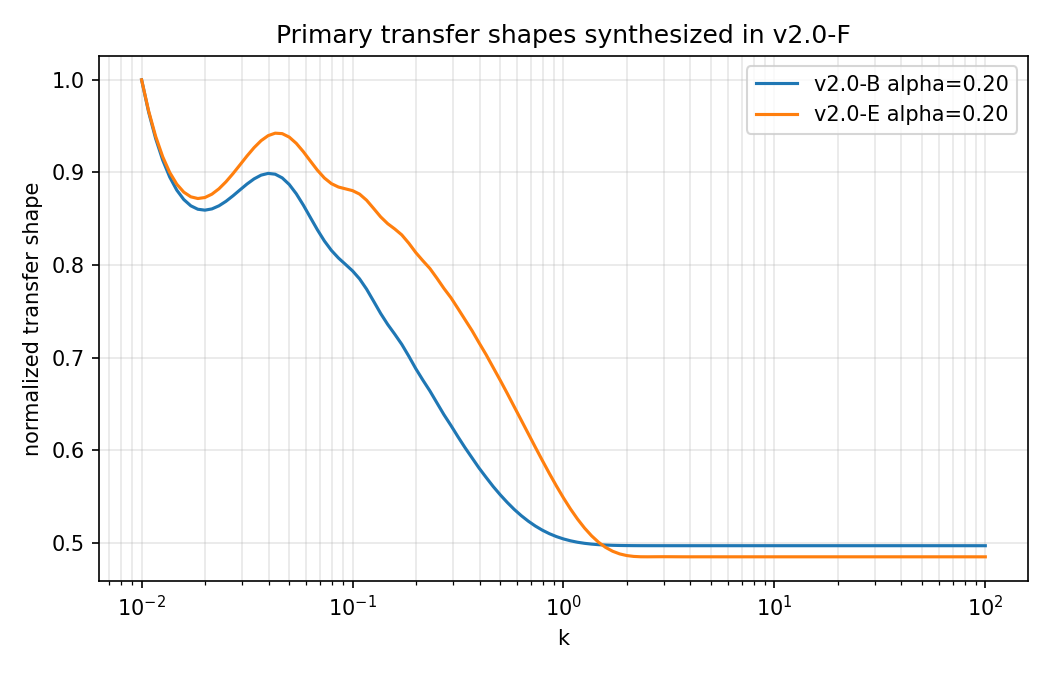
\includegraphics[width=0.92\linewidth]{../figures/SCT_v2_0_F_primary_transfer_comparison.png}
\caption{Primary transfer-shape comparison from v2.0-F. Both preregistered background families show bounded plateau-like behavior rather than gaussian damping.}
\end{figure}

\section{Mechanism identified in v2.1-A}

The plateau is not treated here as a new universal physical effect. For the closed deterministic proxy equation, set
\begin{equation}
V(y)=\frac{a''}{a},\qquad E_k=u_k^2+\left(\frac{u_k'}{k}\right)^2.
\end{equation}
A direct differentiation gives
\begin{equation}
\frac{dE_k}{dy}=\frac{2V(y)u_k u_k'}{k^2}.
\end{equation}
Thus, when $k^2\gg |V(y)|$, the raw transfer is approximately transparent at high $k$, up to oscillatory and order-$k^{-2}$ corrections. Under the v2.0 normalization, the high-$k$ plateau follows from high-$k$ transparency divided by low-$k$ reference amplification:
\begin{equation}
T_{\rm shape, high\text{-}k}\simeq \frac{P_{\rm raw, high\text{-}k}}{P_{\rm raw}(k_{\min})}\simeq \frac{1}{P_{\rm raw}(k_{\min})}.
\end{equation}
This explains why a closed deterministic scattering-style proxy does not naturally produce irreversible gaussian damping.

\section{Mainline transfer-language patch}

The conservative mainline language is now:
\begin{equation}
T_R(k) = \hbox{model-dependent transfer operator.}
\end{equation}
This replaces any presentation in which the gaussian form
\begin{equation}
T_R(k)=\exp[-(k/k_c)^2]
\end{equation}
is treated as the default closed-background expectation.

The branch taxonomy is:
\begin{itemize}
\item \textbf{Closed deterministic background route:} the current evidence from two preregistered toy families points to bounded, plateau-like transfer, not gaussian damping.
\item \textbf{Open-system/diffusive route:} the gaussian kernel remains a conditional toy limit only if an independent dissipative, diffusive, or coarse-graining mechanism is specified.
\item \textbf{Plateau-like closed-route toy branch:} a minimal explanatory form is
\begin{equation}
T_{\rm pl}(k)=p_\infty+\frac{1-p_\infty}{1+(k/k_x)^2},
\end{equation}
where $p_\infty$ is the normalized high-$k$ plateau. This is not a physical universal kernel.
\item \textbf{More physical matching route:} execution remains blocked until a background/action, gauge-invariant variable, $z(\eta)$, matching surface, and matching conditions are independently specified.
\end{itemize}

\section{Claim boundary}

This patch does \emph{not} claim a physical cyclic cosmology, an observational prediction, a no-go theorem for cyclic or bouncing backgrounds, a derived entropy map, or a universal transfer kernel. It records a methodological correction: the gaussian kernel is no longer the conservative default for the closed-background branch.

\section{Public status}

The appropriate public summary is: v1.7--v1.9 are requirements/survey obstruction audits; v2.0 is a limited negative computational result for two preregistered closed-background toy families; v2.1 explains the plateau mechanism and updates the transfer-kernel language accordingly.

\end{document}
